\documentclass[10pt]{article}
\usepackage[utf8]{inputenc}
\usepackage{natbib}
\usepackage[T1]{fontenc}
\usepackage[francais]{babel}
\usepackage{chemist}
\usepackage{array}
\usepackage{amsmath}
\usepackage[squaren,Gray]{SIunits}
\usepackage{numprint}
\usepackage{amsfonts}
\usepackage{amssymb}
\usepackage{graphicx}
\usepackage{mathtools}
\usepackage{fullpage}
\usepackage{mhchem}
\usepackage{listings}
\usepackage{hyperref}


\begin{document}

\section*{Laboratoire d'électrolyse}


Dans le cadre du Projet P3, nous nous concentrons sur la production d'hydrogène sur base de reformage à vapeur.
Il existe évidemment d'autres procédés de production d'hydrogène, dont l'électrolyse. Ce rapport met en avant les
avantages et inconvénients de l'électrolyse, explique le procédé théorique, le montage pratique, et les conclusions 
que nous pouvons tirer des expériences faites en laboratoire.

\subsection*{Avantages et inconvénients}

\paragraph{Avantages} Dans une société où il est devenu impératif de respecter l'environnement, la production 
d'hydrogène par électrolyse semble être une très bonne solution. En effet, ce procédé n'émet pas de gaz à effet de
serre, pour autant que l'électricité soit produite de manière renouvelable; cette manière d'obtenir de l'hydrogène 
deviendrait pérenne\footnote{« Vers une production massive et économique d’hydrogène - Communiqués et dossiers de 
presse - CNRS ». Consulté le 8 novembre 2014. \url{http://www2.cnrs.fr/presse/communique/1570.htm}}. Un autre avantage non 
négligeable est la pureté et la qualité du produit. Un tel procédé permet l'obtention d'hydrogène allant jusqu'à
$99.8 \%$ de pureté.

\paragraph{Inconvénients} L'électrolyse de l'eau nécessite un apport en électricité, dont le coût est bien souvent 
un problème. C'est en grande partie pour cela que ce procédé n'est que très peu utilisé dans le milieu de l'industrie. 
De plus, le rendement d'un tel procédé ne dépasse pas $80 \%$, et il est très difficilement applicable à une production 
à grande échelle\footnote{« AFHYPAC?: Association Française de l’Hydrogène et des Piles à Combustible | Momento de 
l'hydrogène| ». Consulté le 8 novembre 2014. \url{http://www.afhypac.org/fr/accueil}}.

\subsection*{Partie théorique}


L’électrolyse de l’eau consiste en une réaction d’oxydo-réduction forcée durant laquelle on décompose de l’eau (\ce{H_2O})
en dihydrogène (\ce{H_2}) et dioxygène (\ce{O_2}). La réaction globale s’écrit simplement : 

$$\ce{2H2O} \leftrightharpoons \ce{2H2}\uparrow + \ce{O2}\uparrow$$

Cependant, il est difficile de bien comprendre ce qu'il se passe dans le système à partir de cette réaction globale. C’est pourquoi nous travaillerons plutôt avec les demi-réactions mises en jeu.

A la cathode, la réaction de réduction suivante aura lieu:

$$\ce{2H+} + 2 e^{-} \leftrightharpoons \ce{H2}\uparrow  \qquad \text{E\degree = 0 V}$$

Tandis qu’à l’anode, la réaction d’oxydation suivante aura lieu:

$$\ce{2H2O} \leftrightharpoons \ce{O2}\uparrow + 4 e^{-} + \ce{4H+} \qquad \text{E\degree = 1,23 V}$$

On peut ainsi déterminer 2 paramètres intervenant durant une électrolyse : le courant fourni au système et 
l’acidité du milieu\footnote{\url{http://icampus.uclouvain.be/claroline/backends/download.php}}.


\subsection*{Partie expérimentale}

Lors du laboratoire du mercredi 5 novembre, nous avons étudié l'influence de certains paramètres sur le procédé d'électrolyse de l'eau. Chaque groupe a étudié un paramètre afin d'obtenir des résultats dans des conditions différentes. Vous retrouverez ci-dessous les résultats globaux pour la variation du pH, de la température, et du courant.


\begin{figure}[h!]
   \begin{minipage}[c]{.3\linewidth}
      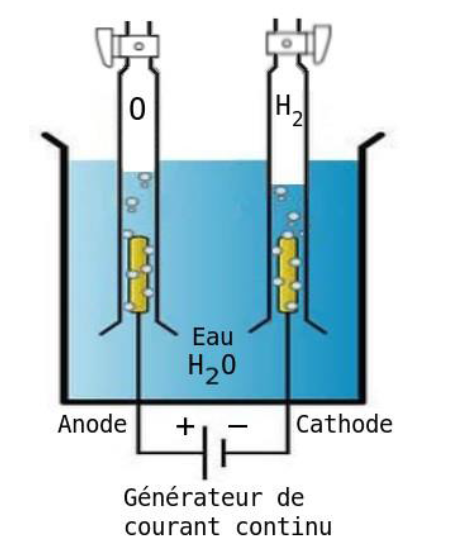
\includegraphics[scale=0.45]{laboelectrolyse.png}
   \end{minipage} \hfill
   \begin{minipage}[c]{.46\linewidth}
      Ci-contre est représenté le montage expérimental pour l'électrolyse de l'eau. En ce qui concerne les 
      électrodes, l'anode est en plomb et la cathode en cuivre. Étant donné que la réaction à la cathode
      nécessite des électrons, c'est la borne négative du générateur de courant qui y sera reliée. La borne 
      positive sera connectée à l'anode vu le dégagement d'électrons.
   \end{minipage}
\end{figure}

\paragraph{Variation du pH}  Différentes expériences ont été réalisées en laboratoire en faisant varier le pH, et
nous nous sommes notamment intéressés aux milieux acides et milieux basiques. Nous observons que le volume de gaz
produit varie linéairement avec le temps, pour un certain pH. Nous observons également que la réaction est favorisée
en milieu très acide, mais également en solution très basique. Nous privilégierons donc des solutions peu diluées.

\paragraph{Variation de la température} Les résultats des expériences à différentes températures sont assez disparates:
dans une expérience, si la température augmente, le temps de production augmente. Dans une autre, le temps de production
diminue; dans une autre encore, le temps augmente puis diminue; et dans la dernière, le temps diminue puis augmente.
Nous ne pouvons pas tirer de conclusions de tels résultats. Cependant, nous remarquons qu'un saut de température important
n'influence pas tellement le temps, donc nous aimerions en déduire qu'il est préférable de travailler à température
ambiante, étant donné qu'il faudrait encore apporter de l'énergie pour modifier cette température. Malheureusement 
nous n'avons des résultats que pour de faibles quantités d'hydrogène produites, et l'écart de temps est sûrement plus 
important pour de plus grandes quantités. Quelques rapides recherches sur internet semblent indiquer qu'une électrolyse
à très haute température peut se révéler intéressante\footnote{« LITEN - Production massive d’H2 par Electrolyse 
Haute Température (EHT) ». Consulté le 10 novembre 2014. \url{http://www-liten.cea.fr/fr/activites_rd/prod_h2_01.htm}}.

\paragraph{Variation du courant} Pour un certain courant, le volume d'hydrogène produit est constant au cours du temps.
Plus le courant augmente, moins il faut de temps pour produire une certaine quantité d'hydrogène. Il apparaît donc 
qu'il faudra augmenter le courant pour accélérer le procédé; et donc augmenter l'apport en électricité. Cela concorde 
avec les recherches antérieures liées aux inconvénients de l'électrolyse.

\subsection*{Conclusions par rapport au projet}

Il nous était demandé de répondre à deux questions à l'issue du laboratoire:
\begin{itemize}
\item Dans quelles conditions opératoires travailleriez-vous pour produire l’hydrogène ?
\item De quelle puissance avez-vous besoin pour le débit d’hydrogène nécessaire à votre production d’ammoniac \unit{1500}{\tonne \per jour} ? 
\end{itemize}
La section précédente nous permet maintenant d'y répondre: les conditions opératoires idéales sont sans doute
de travailler à température ambiante. Effectivement, cela ne requiert pas d'apport d'énergie supplémentaire, et 
les résultats obtenus dans de telles conditions sont tout à fait corrects. Pour l'acidité de la solution nous pouvons
utiliser soit une solution avec un pH très élevé ou avec un pH très faible. En ce qui concerne la puissance, si nous 
voulons atteindre un débit de \unit{1500}{\tonne \per jour}, il nous faut un courant de ... et une tension de ... . La puissance se calcule ensuite à l'aide de la formule $P = U*I$.

\end{document}
